\section{Assignment 2}
In this assignment we study the MCM system of equations, which models the interaction between three species of cells,
tumor-, healthy- and effector cells. The corresponding system of equations is given by
\begin{align*}
    T^{\prime} & =r_1 T\left(1-\frac{T}{k_1}\right)-a_{12} T H-a_{13} T E, \\
    H^{\prime} & =r_2 H\left(1-\frac{H}{k_2}\right)-a_{21} T H, \\
    E^{\prime} & =\frac{r_3 T E}{T+k_3}-a_{31} T E-d_3 E ,
\end{align*}
and its dimensionless form
\begin{align*}
    & x_1^{\prime}=x_1\left(1-x_1\right)-p_1 x_1 x_2-p_2 x_1 x_3, \\
    & x_2^{\prime}=p_3 x_2\left(1-x_2\right)-p_4 x_1 x_2, \\
    & x_3^{\prime}=\frac{p_5 x_1 x_3}{x_1+p_6}-p_7 x_1 x_3-p_8 x_3 .
\end{align*}

The parameters $p_i$ are specified in Table \ref{tab:mcm_parameters}
\begin{table}[H]
    \centering
    \begin{tabular}{|c|c|c|c|}
        \hline
        Parameter   & Definition                & description           & Value \\
        \hline
        $p_1$       & $\frac{a_{12}k_2}{r_1}$     & T->H competition      & 0.5 \\
        $p_2$       & $\frac{a_{31}k_1}{r_1}$     & E->T killing          & 2.5 \\
        $p_3$       & $\frac{r_2}{r_1}      $     & H-T growth ratio      & 0.6 \\
        $p_4$       & $\frac{a_{21}k_1}{r_1}$     & T->H inactivation     & 1.5 \\
        $p_5$       & $\frac{r_3k_2}{r_1}   $     & T->E stimulation      & 4.5 \\
        $p_6$       & $\frac{k_3}{k_1}      $     & E-T capacity ratio    & 1.0 \\
        $p_7$       & $\frac{a_{31}k_3}{r_1}$     & T->E inactivation     & 0.2 \\
        $p_8$       & $\frac{d_3}{r_1}      $     & E natural death       & 0.5 \\
        \hline
    \end{tabular}
    \caption{Parameters of the dimensionless system}
    \label{tab:mcm_parameters}
\end{table}

The goal of this assignment is to study the dynamics of this system as the parameter $p_1$ is varied.
We aim to find the stationary points, bifurcations and (stable) limit cycles of the system, and study their stability.

Additionally, we aim to find the period doubling bifurcations of the limit cycles, and study the stability of the resulting
period-doubled limit cycles. Eventually, we aim to determine the period doubling route to chaos.

\subsection{Stationary points}
Table \ref{tab:mcm_stationary_points} shows the stationary points of the system. 
\begin{table}[H]
	\begin{center}
		\begin{tabular}{|c|c|c|c|c|}
			\hline
			\textbf{index} & $\mathbf{x_1}$ & $\mathbf{x_2}$ & $\mathbf{x_3}$ & \textbf{stability} \\
			\hline
			1 & -2.00 & 6.00 & 0.00 & Unstable \\
			2 & 0.00 & 0.00 & 0.00 & Unstable \\
			3 & 0.00 & 1.00 & 0.00 & Unstable \\
			4 & 1.33$\times 10^{-1}$ & 0.00 & 3.47$\times 10^{-1}$ & Unstable \\
			5 & 1.33$\times 10^{-1}$ & 6.69$\times 10^{-1}$ & 2.13$\times 10^{-1}$ & Stable \\
			6 & 1.00 & 0.00 & 0.00 & Unstable \\
			7 & 1.89$\times 10^{1}$ & -4.62$\times 10^{1}$ & 2.09 & Unstable \\
			8 & 1.89$\times 10^{1}$ & 0.00 & -7.15 & Stable \\
			\hline
		\end{tabular}
	\end{center}
	\caption{Stationary points of the MCM model.}
	\label{tab:mcm_stationary_points}
\end{table}

\subsection{Continuation of stationary points}
We observe two stable stationary points (indices 5 and 8). We continue these
points in the parameter $ p_1 \in [0.5, 1] $ and plot the continuation in Figure \ref{fig:mcm_continuation}.
\begin{figure}[H]
    \centering
    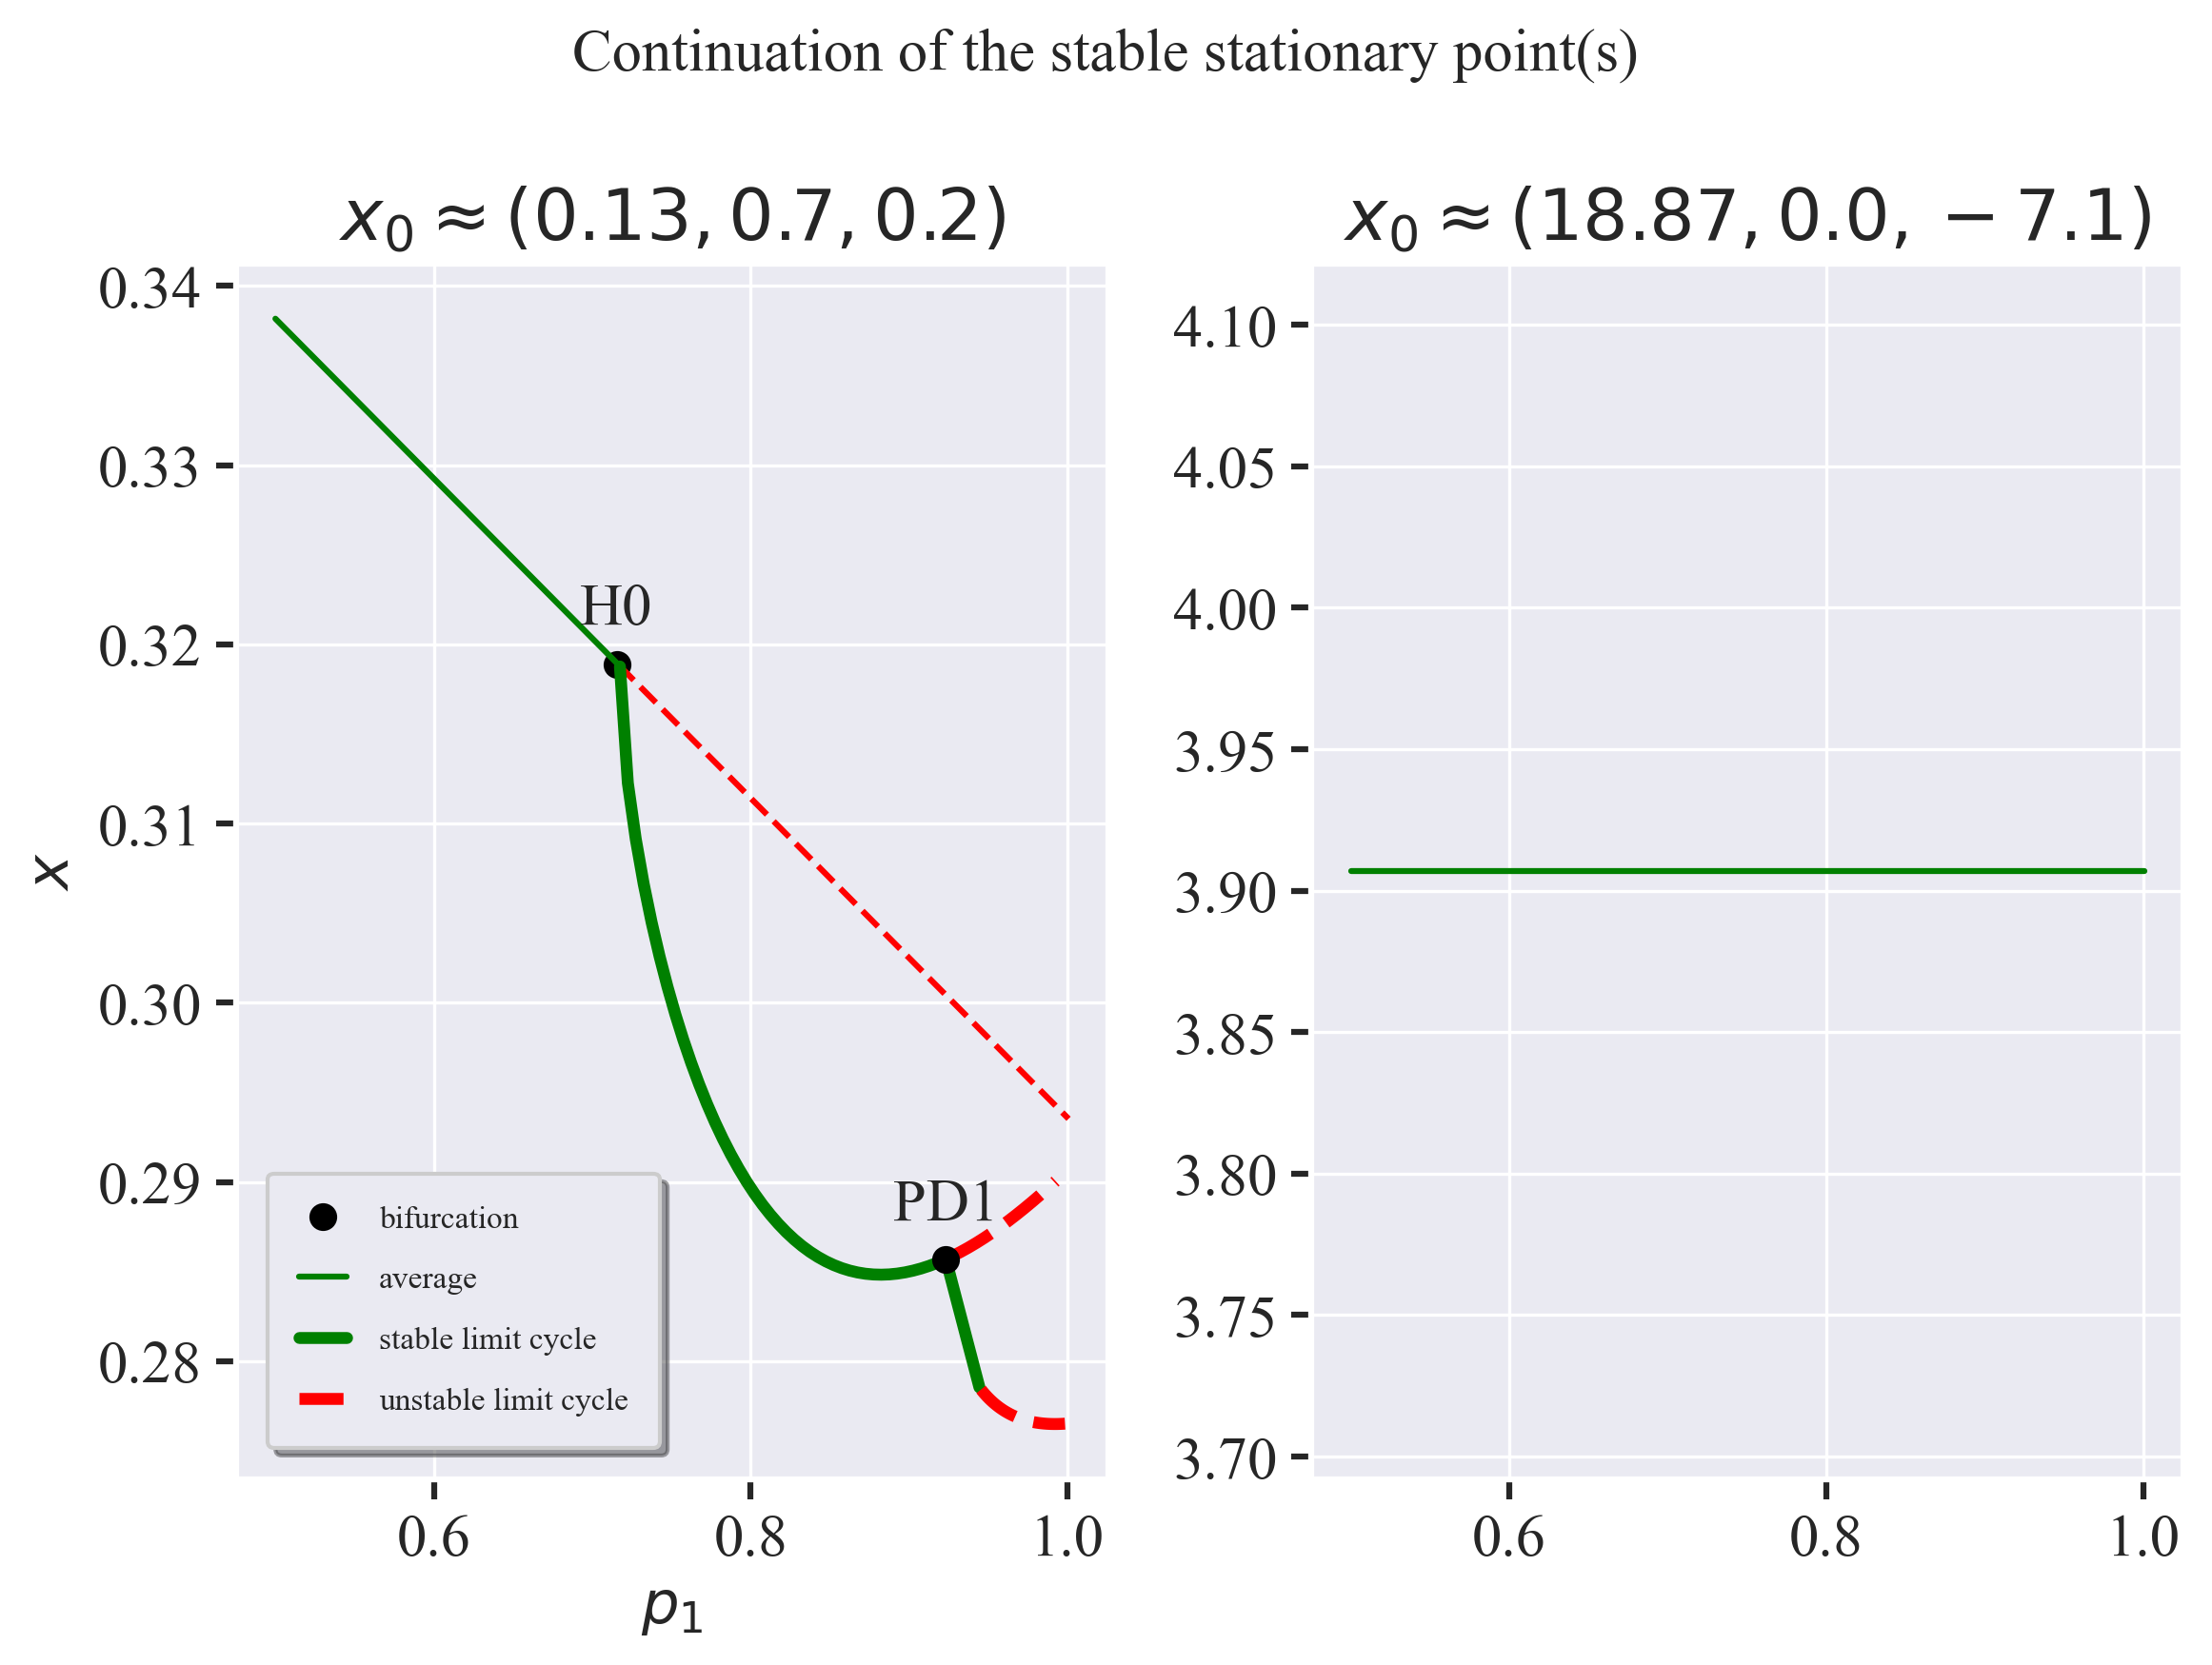
\includegraphics[width=0.8\textwidth]{figures/mcm_continuation.png}
    \caption{Continuation of the stable stationary points in the parameter $p_1$,
    point 5 (left) and point 8 (right). The former encounters a bifurcation at $p_1 \approx 0.71$. From this 
    Hopf-bifurcation an unstable stationary solution and a limit cycle emerges.}
    \label{fig:mcm_continuation}
\end{figure}

The bifurcation that occurs during the continuation of point 5 in Figure \ref{fig:mcm_continuation} is given by
\begin{align*}
    \text{Bifurcation type} & : \text{subcritical?} \ \text{Hopf} \\
    \text{Parameter} & : p_1 \\
    \text{Critical value} & : 0.71 \\
    \text{Eigenvalues} & : 0 \pm 0.36i, -0.53\\
    x_1, x_2, x_3 & : 0.13, 0.67, 0.16
\end{align*}
This bifurcation point was found by applying an indirect method based on the interpolation of test function values, adapted from 
Seydel's book (section 5.3.1). The particular test function used was the maximum of the real part of the eigenvalues of
the system Jacobian.

The bifurcation is a Hopf-bifurcation, as a complex pair of eigenvalues crosses the imaginary axis with non-zero velocity
That is to say, the eigenvalues of the system jacobian at the continuation step dircetly after the bifurcation are
\begin{align*}
    0.007 \pm 0.355i, -0.54,
\end{align*}
which shows the eigenvalues pases through the imaginary axis with non-zero velocity.

From the hopf bifurcation we determine the first dynamical solution using the method described in 
section 7.6.2 of Seydel's book. In other words we solve the following BVP 
\begin{align*}
    \left(\begin{array}{l}
        \mathbf{x} \\
        T \\
        \lambda \\
        \mathbf{h}
        \end{array}\right)^{\prime}=\left(\begin{array}{c}
        T \mathbf{f}(\mathbf{x}, \lambda) \\
        0 \\
        0 \\
        T \mathbf{f}_{\mathbf{x}}(\mathbf{x}, \lambda) \mathbf{h}
        \end{array}\right), \quad\left(\begin{array}{c}
        \mathbf{x}(0)-\mathbf{x}(1) \\
        \mathbf{h}(0)-\mathbf{h}(1) \\
        \sum_i h_i \partial f_1 / \partial x_i \\
        h_1(0)-1
        \end{array}\right)=\mathbf{0},
\end{align*}
using the shooting method in order to switch from the stationary solution to the limit cycle. 
The solution we obtain is
\begin{align*}
    \mathbf{x}^{(0)} & = (0.13, 0.67, 0.15)\\
    T^{(0)} &= 17.6\\
    p_1^{(0)} & = 0.72 \\
    \mathbf{h}^{(0)} &= (1.00, -1.40 , 0.00),
\end{align*}
from which we get an estimate for the period of the limit cycle.

\subsection{Continuation of limit cycle}
We use the solution of the BVP from the previous section as an initial guess for the continuation of the limit cycle.
Following the method outlined in section 7.6.3 of Seydel's book, we repeatedly solve the BVP, wherein each 
iteration starts with the solution of the previous iteration plus a small perturbation given 
by $\mathbf{h}$ (Equation 7.24, Seydel)
\[
    \bar{\mathbf{x}}^{(k+1)} = \mathbf{x}^{(k)} + \delta \mathbf{h}^{(k)}, \quad \bar{T}^{k+1} = T^{k}, \quad \bar{p}_1^{(k+1)} = p_1^{(k)},
\]
for a suitably small parameter $\delta \approx 0.13$. This results a sequence of limit cycles starting from the Hopf point (k=0)
\[
    \textrm{cycle}^{(k)} = \left\{\mathbf{x}^{(k)}, T^{(k)}, p_1^{(k)} \right\}, \quad k = 0, 1, 2, \ldots
\]
which we integrate over their respective periods and plot in Figure \ref{fig:mcm_limit_cycle_continuation}.
\begin{figure}[H]
    \centering
    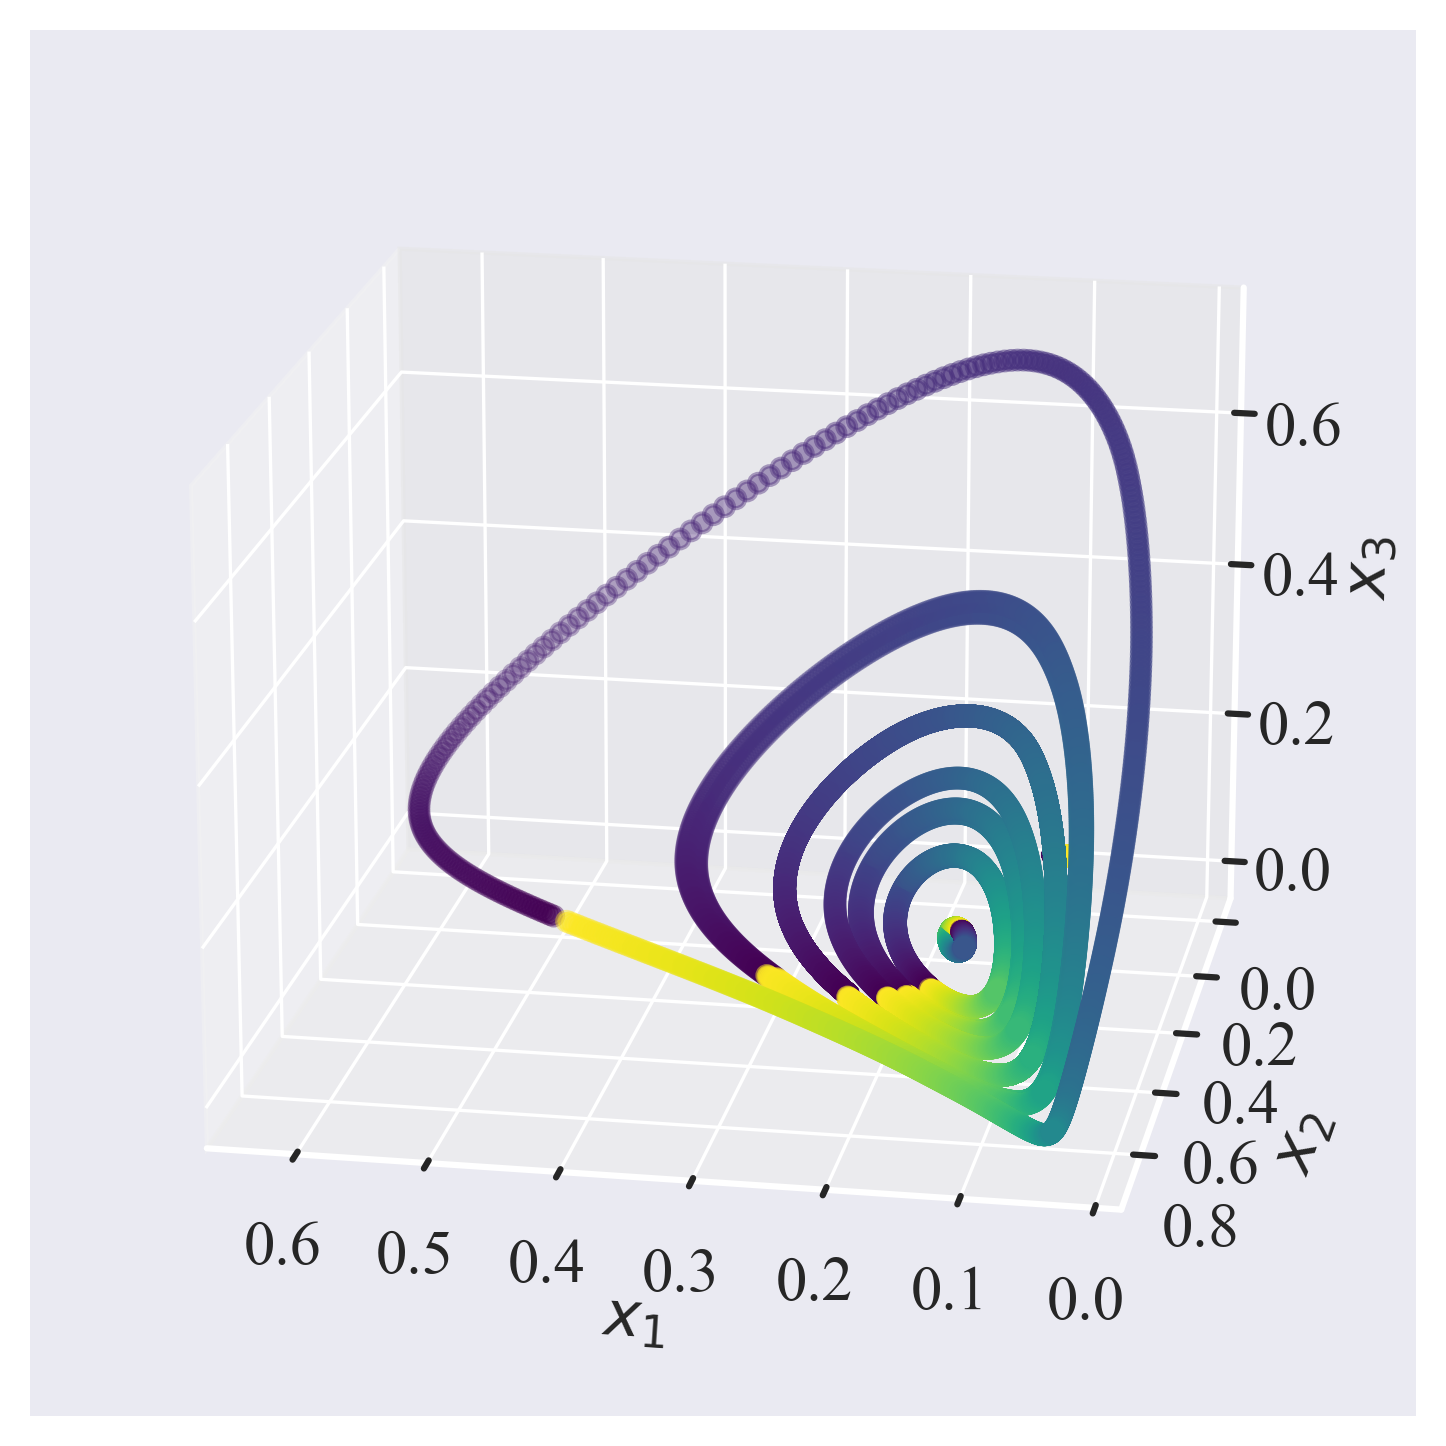
\includegraphics[width=0.7\textwidth]{figures/mcm_limit_cycles2.png}
    \caption{Continuation of the limit cycle in the parameter $p_1$. The colors indicate the the flow of time
    from dark to light.}
    \label{fig:mcm_limit_cycle_continuation}
\end{figure}
The limit cycles in Figure \ref{fig:mcm_limit_cycle_continuation} are averaged both in time and in space to obtain the points in 
Figure \ref{fig:mcm_limit_cycle_continuation}.

For each limit cycle we calculate the monodromy matrix $M$ using Algorithm 7.12
from section 7.5.1 of Seydel. The eigenvalues of $M$ (Floquet multipliers) $\mu_j$ are then used to determine the stability of the limit cycle
(according to Summary 7.5, p. 315, Seydel).

The stability of the limit cycles obtained from this process is accordigly shown in Figure \ref{fig:mcm_continuation}, where 
red and green crosses indicate unstable and stable limit cycles, respectively. 

At this point we observe something unexpected. The limit cycles are all unstable, which is not what we would expect from the
Hopf-bifurcation. This is likely due to an incorrectly calculated monodromy matrix. 
This hinders our progress in finding the period-doubling bifurcations and the route to chaos, as will become apparent in the next section.

\subsection{Period doubling bifurcations}
Period doubling bifurcations occur at those limit cycles where there is a $j$ for which $\mu_j = -1$.
Hence, we continue the limit cycle (and calculate the monodromy matrices) until we find a multiplier close to $-1$. Then, we apply the
shooting method to solve the BVP in Equation 7.27 of Seydel's book. This gives a point
either on original branch or on the period-doubled branch, depending on how we choose the boundary conditions
and what kind of symmetry we expect (section 6.4, Seydel). 

Once we have the period-doubled branch, we can continue it in the same way as the original branch. That is using the continuation method
from the previous section and the solution to the BVP 7.27. We continue until
we find a second period-doubling bifurcation, and so on. 

Alternatively, we can predict the parameter values at which we expect period-doublings 
to occur using Feigenbaum's law (Equation 7.14, Seydel)
\[
    \lim_{n \to \infty} \frac{p_{n+1} - p_n}{p_{n} - p_{n-1}} = 0.21416 \dots,
\]

\subsection{Conclusion}
In the above treatment of the MCM system we 
\begin{enumerate}
    \item Found the stationary points of the system and continued the stable ones in the parameter $p_1$;
    \item Found a Hopf-bifurcation at $p_1 \approx 0.71$ and calculated the first limit cycle using the shooting method;
    \item Continued the limit cycle in the parameter $p_1$ and calculated the stability of the limit cycles;
    \item Described a method for finding period-doubling bifurcations and/or predicting them.
\end{enumerate}

We have yet
\begin{enumerate}
    \item To find the period-doubling bifurcations of the limit cycles and study the stability of the resulting
    period-doubled limit cycles;
    \item To determine the period doubling route to chaos.
\end{enumerate}

The reason for these unexplored parts is (probably) due to an incorrectly calculated monodromy matrix,
which results in an incorrect stability analysis of the limit cycles. This hindered our progress
in finding the period-doubling bifurcations and the route to chaos, since the proposed method
for doing so assumed good approximations of the monodromy matrix.